In diesem Kapitel werden zunächst die Grundlagen und die Definition der Datenbank erläutert. In den weiteren Kapiteln wird ein Vergleich zwischen relationalen und objektorientierten Datenbanken aufgestellt und wie es zu der Entscheidung für MongoDB gekommen ist. Des Weiteren geht es um die Performance der Abfragen gehen und auf die Lösung mittels Cron-Jobs und die Implementierung eingegangen.

\section{Grundlagen (F)}
\setauthor{Felix Arzt}
"Eine Datenbank ist eine organisierte Sammlung von strukturierten Informationen oder Daten, die typischerweise elektronisch in einem Computersystem gespeichert sind. Eine Datenbank wird normalerweise von einem Datenbankverwaltungssystem (DBMS) gesteuert."
\newline
(\url{https://www.oracle.com/de/database/what-is-database/#:~:text=Eine%20Datenbank%20ist%20eine%20organisierte,einem%20Datenbankverwaltungssystem%20(DBMS)%20gesteuert.}; Zugriff: 20.02.2024)
\newline
Dabei gibt es verschiedene Arten von Datenbanktypen. Im Zuge dieser Diplomarbeit wird lediglich die relationale und die objektorentierte Datenbank von Relevanz. Im folgenden Kapitel wird nun näher auf den Unterschied zwischen den beiden Typen eingegangen wird auf die Gründe, warum es zur Entscheidung für MongoDB gekommen ist.
\cite{database_basics}

\section{Vergleich (F)}
\setauthor{Felix Arzt}
\textbf{Relationale Datenbank}
\newline
Eine relationale Datenbank basiert auf einem relationalen Modell und stellt die Daten in einer Tabelle dar. Dabei ist jede Zeile in dieser Tabelle genau ein Datensatz, welcher mit einer eindeutigen ID (Schlüssel) versehen ist. Die Spalten der Tabelle stellen die Attribute dar, welche gespeichert werden können. Bei einer relationalen Datenbank sind die logischen Datenstrukturen, sprich die Datentabellen, Ansichten und Indizes, von den physischen Datenstrukturen getrennt. Dies ermöglicht es den Datenbankadministrator bzw. die Datenbankadministratorin physische Datenstrukturen zu verändern ohne dabei die logische Datenstruktur zu beeinträchtigen. 
\newline
Der wohl größte Vorteil einer relationalen Datenbank ist die \textbf{ACID-Eigenschaft}, dabei steht ACID für: \textbf{A}tomicity, \textbf{C}onsistency, \textbf{I}solation und \textbf{D}urability.

\begin{itemize}
    \item \textbf{Atomicity}
        \newline
        Atomicity beschreibt, dass entweder die Transaktion als ganzes durchgeführt wird, oder gar nicht. Das bedeutet, sollte ein Teil der Transaktion fehlerhaft sein, wird alles zurückgesetzt und nichts persistiert. Nur wenn alle Abschnitte der Transaktion erfolgreich waren, werden die Daten persistiert.
    \item \textbf{Consistency}
        \newline
       Consistency beschreibt den Zustand der Daten. Das Ziel einer relationalen Datenbank ist, dass diese immer im Konsistenten Zustand sind, das bedeutet, dass sie allen Regeln der Datenbank entsprechen und zu jeder Zeit und auf allen Instanzen (Kopien der Datenbank) dem neuesten Stand entsprechen.
    \item \textbf{Isolation}
        \newline
        Isolation beschreibt den Vorgang, dass jede Transaktion verborgen von den anderen abläuft und erst nach beenden der Transaktion in der Datenbank "veröffentlicht" wird. Dadurch wird verhindert, dass sich die Transaktionen gegenseitig beeinflussen bzw. beeinträchtigen und trotzdem parallel ablaufen können.
    \item \textbf{Durability}
        \newline
        Durability ist die Versicherung, dass alle Daten dauerhaft gespeichert werden, sobald die Transaktion abgeschlossen ist.
\end{itemize}
Zusammenfassend lässt sich sagen, dass eine relationale Datenbank besonders geeignet ist, wenn eine Vielzahl von Daten in einer sicheren, regelbasierten (Atomicity) und konsistenten (Consistency) Weise gespeichert werden sollen, insbesondere wenn diese Daten untereinander in Beziehung stehen. In diesem speziellen Fall der vorliegenden Diplomarbeit war dies durchaus eine Anforderung, da zahlreiche Daten gespeichert werden mussten und eine klare Beziehung zwischen den einzelnen Tabellen vorhanden war.
\newline
Trotz dieser Anforderungen entschied sich das Projektteam aufgrund des umfangreichen Know-Hows in der Kollaborationsfirma für den Einsatz von objektorientierten Datenbanken. Diese Entscheidung führte zur Auswahl von MongoDB als Datenbanktyp, da die benötigten Daten bereits in einer MongoDB-Datenbank gespeichert waren. Ein Wechsel zu einer relationalen Datenbank wäre aufgrund des damit verbundenen Aufwands nicht gerechtfertigt gewesen.
\newline
Rückblickend ist anzumerken, dass sich mit der Verwendung einer relationalen Datenbank viele Abfragen wesentlich einfacher gestaltet hätten. Einige Abfragen erforderten in MongoDB die Durchführung eines JOINs über zwei Collections, was sich als durchaus anspruchsvoll erwies.
\cite{database_relational}
\newline
\begin{figure}[h!]
  \centering
  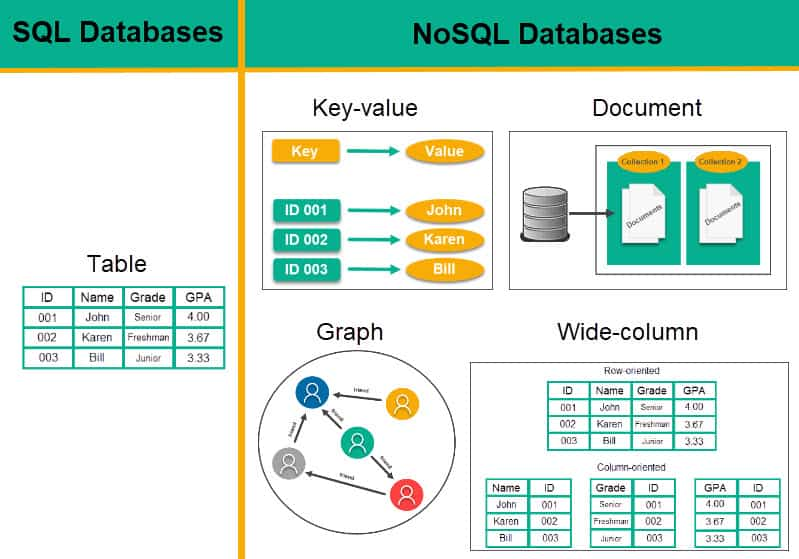
\includegraphics[width=0.8\textwidth]{pics/database-types.jpg}
  \caption{Relational vs. Objektorientiert}
  \cite{database_types}
\end{figure}

\section{MongoDB (F)}
\setauthor{Felix Arzt}
\begin{figure}[h!]
    \centering
    
\includegraphics[width=0.8\textwidth]{pics/mongodb.png}
    \caption{MongoDB Logo}
    \cite{database_mongodb_logo}
    \label{fig:enter-label}
\end{figure}

\subsubsection{Grundlagen}
MongoDB ist eine dokumentenbasierte Datenbank, die für eine einfache Anwendungsentwicklung und Skalierung ausgelegt ist. Dabei gibt es drei verschiedene Möglichkeiten MongoDB zu verwenden: 
\begin{itemize}
    \item \textbf{MongoDB Atlas}
        \newline
        Dieses ist ein Multi-Cloud Datenbankdienst, welcher das Deployen und Verwalten der Datenbank vereinfacht, aber gleichzeitig die Vielseitigkeit bietet, die zum Erstellen von leistungsstarken Anwendungen benötigt werden.
    \item \textbf{MongoDB Enterprise}
        \newline
        Dies ist ein abonnementbasierte und selbstverwaltete Version von MongoDB und umfasst mehr Funktionen:
        \begin{itemize}
            \item \textbf{LDAP-Authentifizierung}
                \newline
                LDAP bedeutet "lightweight directory access protocol" und hilft Benutzern beim Finden von Daten über Organisationen und Personen. LDAP-Authentifikation verfolgt dabei folgende Ziele: Daten im LDAP Vezeichnis zu speichern und Benutzer beim Zugriff auf dieses Verzeichnis zu authentifizieren. Dabei ist LDAP eines der wichtigsten Authentifizierungsprotokolle, welches für Verzeichnisdienste entwickelt wurde.
                \cite{ldap_auth}
            \item \textbf{Kerberos Authentifizierung}
                \newline
                Ist ein Sicherheitsprotkoll, welches mit dem KDC (Key Distribution Center) arbeitet, welches alle Clients, User und Dienste verwenden müssen, um zu authentifizieren. Außerdem wird beim Authentifizierungsprozess ein KDC-Ticket vergeben. Dieses Authentifizierungsverfahren ist die Standardmethode für das Betriebssystem Microsoft Windows.
                \cite{kerberos_auth}
            \item \textbf{Audit Events}
                \newline
                Audit-Events sind sicherheitsrelevante Ereignisse in einem System zum Beispiel ein Verstoß gegen Systemzugriffskontroll- oder Verantwortlichkeitssicherheitsrichtlinien und melden diese Verstöße an den System-Audit-Logger, welcher als Teil des Kernels ausgeführt wird. Es werden Name des Ereignisses, Erfolg oder Misserfolg und alle anderen ereignisspezifischen Informationen übermittelt.
                \cite{audit_events}
\end{itemize}
    \item \textbf{MongoDB Community}
        \newline
        Dies ist der Source Code von MongoDB, welcher kostenlos und selbstverwaltet zur Verfügung steht.
\end{itemize}
\cite{mongodb_basics}

\subsubsection{Aufbau der Datenbank}
Die Datenbank ist in folgende Teile unterteilt:

\begin{itemize}
    \item \textbf{Fields}
        \newline
        Dies sind die kleinste Einheit in der Datenstruktur und würden in einer relationalen Datenbank einer Entität ensprechen.
    \item \textbf{Documents}
        \newline
        Documents entsprechen in einer relationalen Datenbank einem Datensatz und werden mittels BSON (Binary JSON) kodiert. Im Vergleich zu JSON ist es allein durch die visuelle Inspektion der beiden Formate nicht möglich, einen Unterschied festzustellen, da BSON auf dem JSON-Format aufbaut.
        \newline
        Der entscheidende Unterschied zwischen BSON und JSON liegt darin, dass BSON zusätzliche Datenformate wie Datumswerte und Binärdaten unterstützt. Dies wird durch kodierte Typ- und Längeninformationen ermöglicht, was wiederum zu einer erheblichen Leistungssteigerung beim Durchlaufen des Datensatzes führt. Die Integration von BSON ermöglicht es auch, Arrays und andere Dokumente effizient in diese Datensätze einzufügen.
        \newline
        Der Vorteil von "Documents" sind:
        \begin{itemize}
            \item Dokumente entsprechen in einigen Programmiersprachen nativen Datentypen
            \item Die Einbindung von Arrays und Documents vermeidet aufwendige JOINS
            \item Durch das dynamische Schema kann man die Datenbankstruktur sehr vielseitig gestalten
        \end{itemize}
        \begin{figure}[h!]
            \centering
            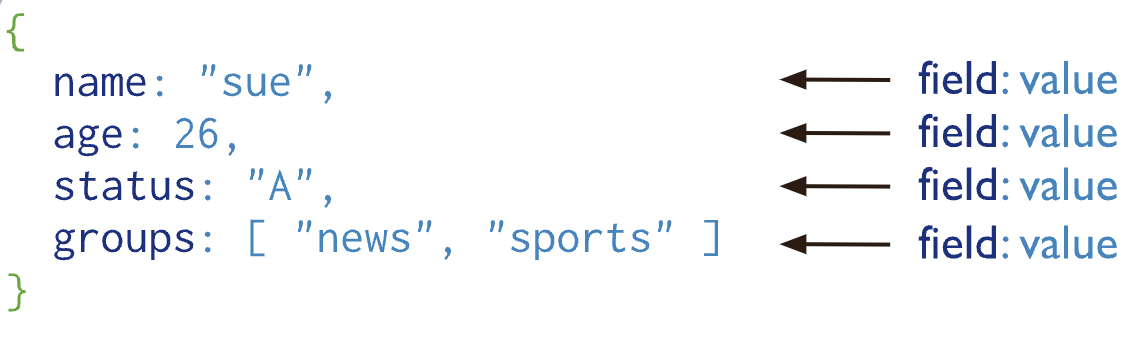
\includegraphics[width=0.8\textwidth]{pics/document.png}
            \caption{Document in MongoDB}
            \cite{mongodb_document}
            \label{fig:enter-label}
        \end{figure}
        \cite{mongodb_json_vs_bson}
    \item \textbf{Collections}
        \newline
        Die "Documents" werden in sogenannten "Collections" gespeichert, welche vergleichbar mit Tabellen in relationalen Datenbanken sind. Collections besitzen eine sogenannte "dynamic schema" Eigenschaft, was bedeutet, dass "Documents" in einer "Collection" unterschiedliche "Fields" besitzen können. Wie man im unten gezeigten Beispiel sieht, können beide dieser Documents in der selben Collection gespeichert werden.
        \begin{lstlisting}
            {"username": "admin", "firstname": "John"}
            {"lastname": "Doe"}
        \end{lstlisting}
        Man könnte also ausschließlich mit einer einzigen Collection arbeiten und in diese alle Datensätze speichern, man würde allerdings ziemlich schnell an seine Grenzen stoßen.
    \item \textbf{Cluster}
        \newline
        In einem Cluster sind alle Server der Datenbank gespeichert in denen sich die Collections befinden. Diese Cluster können Replica Sets sein, also Kopien aller Daten, oder Sharded-Cluster sein. Zu diesem Cluster wird im Laufe dieses Kapitels noch genauer eingegangen.
        \cite{mongodb_collections}
\end{itemize}

\subsubsection{Skalierung}
Die die Anzahl der Daten die gespeichert werden im Laufe der Zeit immer weiter anwächst, ist es wichtig seine Datenbank einfach skalieren zu können. 

\subsubsection{Horizontale Skalierung}
MongoDB wurde auf die horizontale Skalierung ausgelegt. Dazu müssen neue Maschinen (Server) dazugekauft werden, auf denen anschließend die Daten verteilt werden. Durch das dokumentenbasierte Datenmodell ist es wesentlich einfacher die Daten auf verschiedene Maschinen zu verteilen, dabei achtet MongoDB selbst darauf, dass alle Server annähernd gleich ausgelastet sind. Dazu werden Daten auch von einem Server auf einen anderen Server verschoben. Dazu verwendet MongoDB Shard-Schlüssel, welcher als Field in den Documents gespeichert wird und dient dazu die Documents in den Collections zu verteilen.
\cite{mongodb_collections}

Wie in der untenstehenden Grafik zu sehen, wird hier von "Shards" gesprochen. Das sogenannte Sharding stammt aus der Welt der traditionellen Datenbanken und beschreibt das zerteilen einer großen Datenbank in mehrere kleine. Die neu entstandenen kleinen Datenbanken nennt man Shards. Der Vorteil dieser Methode sind schnellere Schreib- und Lesezugriffe, da alle Shards in einem Cluster diese Befehle ausführen, wodurch ein hoher Grad der Parallelität erreicht wird.
\begin{figure}[h!]
    \centering
    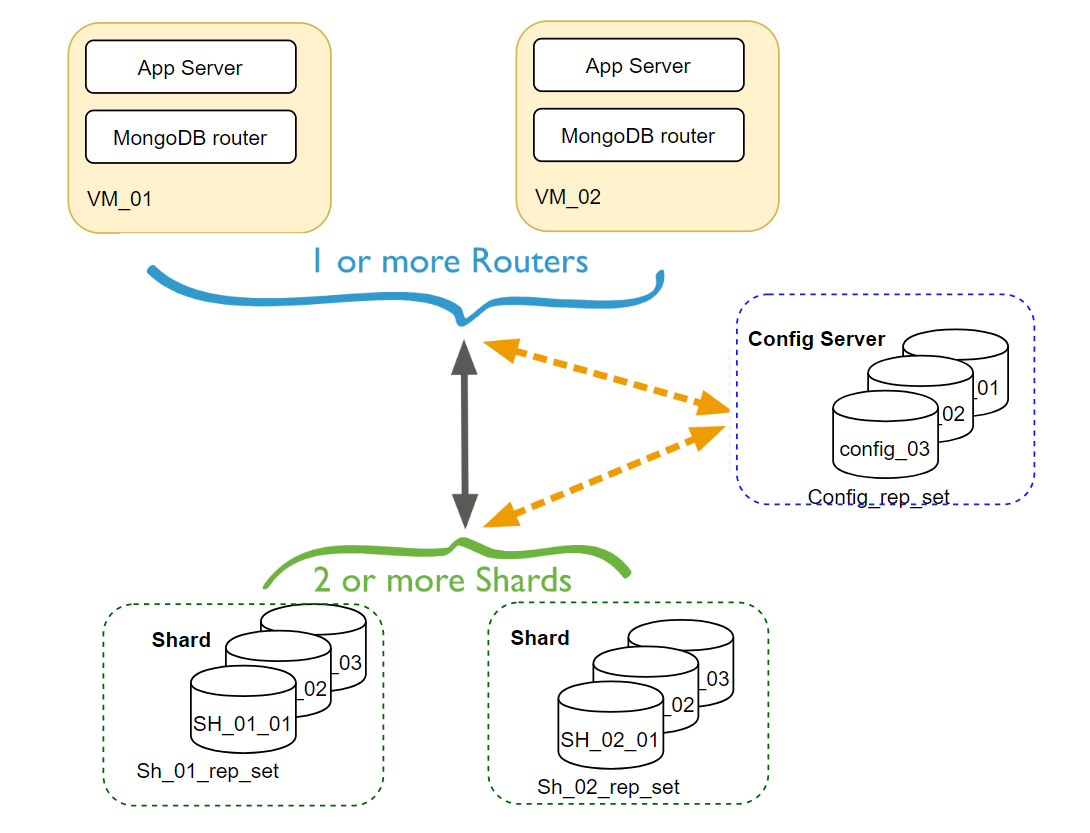
\includegraphics[width=0.6\textwidth]{pics/vertical_scaling_mongodb.png}
    \caption{Horizontale Skalierung MongoDB}
    \cite{vertical_scaling_mongodb}
    \label{fig:enter-label}
\end{figure}
\newline
MongoDB unterstützt zwei unterschiedliche Sharding-Methoden:
\begin{itemize}
    \item \textbf{Hashed Sharding}
        \newline
        Bei dieser Methode wird ein Hashwert aus dem Shard-Schlüssel gebildet und anschließend wird jedem Block ein Bereich zugewiesen, der auf den gehashten Wert basiert.
        \begin{figure}[h!]
            \centering
            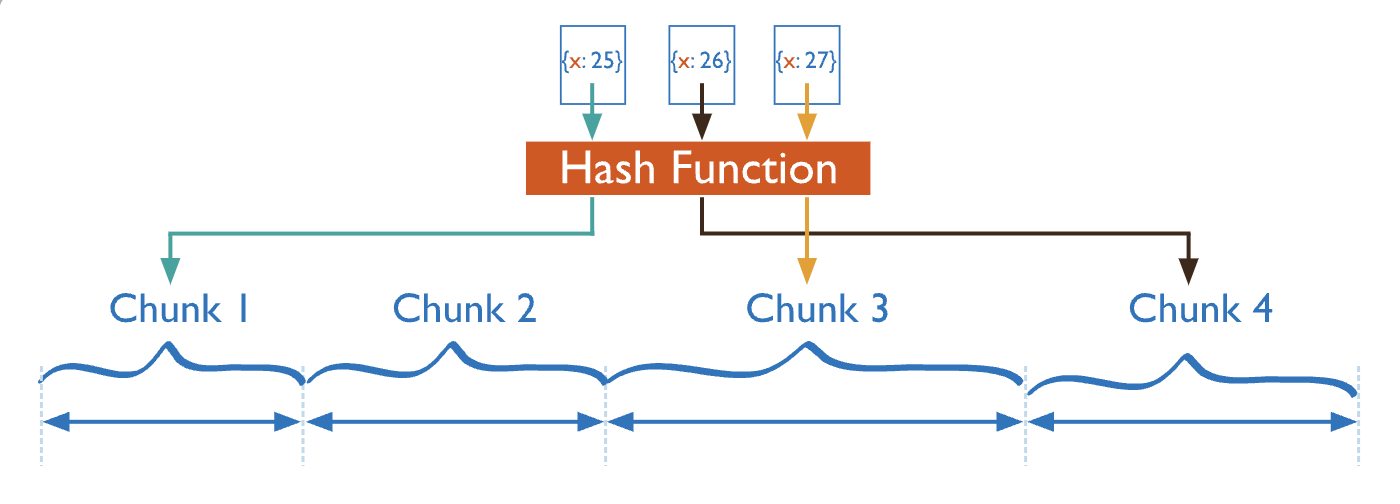
\includegraphics[width=0.5\textwidth]{pics/hashed_sharding.png}
            \caption{Hashed Sharding MongoDB}
            \cite{hashed_sharding_image}
            \label{fig:enter-label}
        \end{figure}
    \item \textbf{Ranged Sharding}
        \newline
        Bei dieser Methode werden die Daten aufgrund der Shard Schlüsselwerten in Bereiche unterteilt. Anschließend wird auf Basis der Shard-Schlüsselwerte  jedem Chunk ein entsprechender Bereich zugewiesen.
        \begin{figure}[h!]
            \centering
            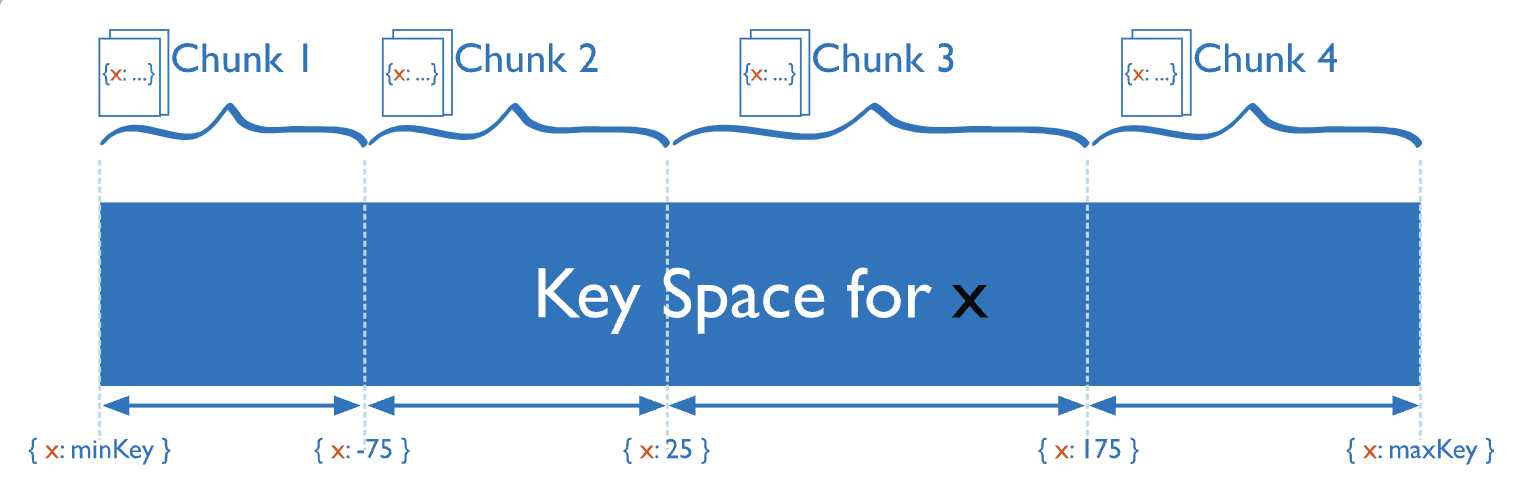
\includegraphics[width=0.5\textwidth]{pics/ranged_sharding.png}
            \caption{Ranged Sharding MongoDB}
            \cite{range_sharding_image}
            \label{fig:enter-label}
        \end{figure}
\end{itemize}

\subsubsection{Vertikale Skalierung}
Es gibt allerdings auch die Möglichkeit eine MongoDB Datenbank vertikal zu Skalieren. Dabei wird die Kapazität eines einzigen Servers gesteigert, indem man eine stärkere CPU, mehr RAM oder mehr Speicherplatz einbaut. In diesem Fall ist man allerdings an den technologischen Fortschritt angewiesen und es ist nicht unendlich möglich diese Skalierungsvariante zu verwenden. Des weiteren ist in den meisten Fällen eine horizontale Skalierung wesentlich kosteneffizienter als eine vertikale.
\cite{mongodb_sharding}

\subsubsection{Abfragen in MongoDB}
Dadurch, dass MongoDB keine relationale Datenbank ist, sehen die Abfragen auch anders aus wie bei SQL-basierte Datenbanken. In diesem Abschnitt wird auf die grundlegenden Abfragen in Kombination mit einem JavaScript Backend eingegangen. Bevor man allerdings mit den Abfragen beginnen kann, muss man zuerst eine Verbindung zur Datenbank aufbauen. Im untenstehenden Beispiel ist gezeigt wie dieser Verbinungsaufbau im Fall eines express.js Backends funktioniert.
\begin{lstlisting}
    const client = new MongoClient('<connection_string>')
    const result = client.connect()
    const db = result.db('<collection_name>')
\end{lstlisting}
Da nun die Verbindung zur Datenbank beseteht und eine Collection ausgewählt wurde (Zeile 3, obiger Codesnippet) kann man mit den Abfragen beginnen.
\newline
Möchte man aus einer Collection, Documents abfragen, gibt es zwei verschiedene Varianten, dies zu machen. Sind "einfache" Abfragen, wie zum Beispiel vergleiche von einzelnen oder mehreren Fields notwendig, benötigt es die "find"-Methode. In der "find"-Methode kann man die Query, in Form eines Objekts übergeben, lässt man es allerdings leer, werden alle Documents aus der Collection zurückgegeben.
\begin{lstlisting}
    const res1 = await db.collection.find({}).toArray()
    const res1 = await db.collection.find(
        {
            "firstname": "John"
        }
    ).toArray()
\end{lstlisting}
Wie im obigen Beispiel zu sehen ist, benötigt es nach der find-Methode eine weitere Methode, um das Ergebnis anzeigen zu können. Von diesen Methoden gibt es mehrere, anbei sind die zu finden, welche in dieser Diplomarbeit verwendet wurden.
\begin{center}
    \begin{tabular}{ | m{3cm} | m{2.3cm}| m{8cm} | } 
        \hline
        Name & Übergabetyp & Beschreibung \\ [0.5ex] 
        \hline\hline
        limit & number & Limitiert Documents die zurückgegeben werden \\
        \hline
        sort & object & Sortiert Documents nach Field z.B. \{'<field>': 1\} \\
        \hline
        project & object & Fields die zurückgegeben werden \\
        \hline
        skip & number & Überspringt n Documents \\
        \hline
    \end{tabular}
\end{center}
\cite{mongodb_query_methods}
Es können noch andere Methoden definiert werden, weitere Methoden sind im folgenden Link zu finden.
\newline
\url{https://mongodb.github.io/node-mongodb-native/3.6/api/Collection.html#find}
\newline
Um die Abfragen spezifischer zu gestalten, kann man auf verschiedene Operatoren zugreifen. Folgende Operatoren gibt es in MongoDB:
\begin{center}
    \begin{tabular}{ | m{1.5cm} | m{13cm} | } 
        \hline
        Name & Beschreibung \\ [0.5ex] 
        \hline\hline
        \$eq & Matches values that are equal to a specified value \\
        \hline
        \$gt & Matches values that are greater than a specified value \\
        \hline
        \$gte & Matches values that are greater than or equal to a specified value \\
        \hline
        \$in & Matches any of the values specified in an array \\
        \hline
        \$lt & Matches values that are less than a specified value \\
        \hline
        \$lte & Matches values that are less than or equal to a specified value \\
        \hline
        \$ne & Matches all values that are not equal to a specified value \\
        \hline
        \$nin & Matches none of the values specified in an array \\
        \hline
        \$and & Joins query clauses with a logical AND returns all documents that match the conditions of both clauses \\
        \hline
        \$not & Inverts the effect of a query expression and returns documents that do not match the query expression \\
        \hline
        \$nor & Joins query clauses with a logical NOR returns all documents that fail to match both clauses \\
    \end{tabular}
\end{center}
\begin{center}
    \begin{tabular}{ | m{1.5cm} | m{13cm} | } 
        \$or & Joins query clauses with a logical OR returns all documents that match the conditions of either clause \\
        \hline
        \$exists & Matches documents that have the specified field \\
        \hline
        \$type & Selects documents if a field is of the specified type \\
        \hline
        \$regex & Selects documents where values match a specified regular expression \\
        \hline
    \end{tabular}
\end{center}
\cite{mongodb_query_operations}
\newline
Die Syntax um oben dargestellten Befehle zu verwenden sieht wie folgt aus:
\newline
\begin{lstlisting}
    const res = await db.collection.find(
        {
            "firstname": { $exists: true }
        }
    ).toArray()

    const res1 = await db.collection.find(
        {
            $and: [
                "firstname": { $exists: true },
                "lastname": "Doe"
            ]
        }
    ).toArray()
\end{lstlisting}
\cite{mongodb_query_basics}
\newline
Möchte man nun allerdings nicht nur "einfache" Vergleichsabfragen durchführen, sondern möchte Documents gruppieren, oder einen Join auf eine andere Collection machen, benötigt man die Aggregation-Operation. Diese Operationen verarbeiten mehrere Documents, aus verschiedenen Collections, und können Berechnungen dieser Documents zurück geben. Es gibt zwei verschiedene Arten von Aggregation-Operationen:
\begin{itemize}
    \item \textbf{Aggregation Pipelines}
        \newline
         Eine Aggregation-Pipeline besteht aus einem oder mehreren Phasen, welche die Documents durchlaufen:
        \begin{itemize}
            \item In jeder Phase wird eine Operation an dem Document durchgeführt.
            \item Die Documents welche von einer Phase ausgegeben werden, werden an die nächste Phase übergeben.
            \item Gibt ein gruppiertes Ergebnis zurück, in dem man ein Minimum, Maximum, Durchschnitt oder Gesamtergebnis berechnen kann.
        \end{itemize}
        Im folgenden Beispiel wird eine Aggregation gezeigt, welche aus zwei Phasen besteht. Dabei filtert die ersten Phase die Bestellungen nach ihrer Größe und gibt alle Bestellungen an die nächste Phase weiter, welche die Größe Medium besitzen. In der zweiten Phase werden die übergeben Documents gruppiert und die Anzahl summiert.
        \begin{lstlisting}
            db.orders.aggregate( [
                // Phase 1
               {
                  $match: { size: "medium" }
               },
            
               // Phase 2
               {
                  $group: { _id: "$name", totalQuantity: { $sum: "$quantity" } }
               }
            ] )
        \end{lstlisting}
    \item \textbf{Single Purpose Aggregation Methods}
        \newline
        Diese Aggregation verarbeiten nur Documente aus einer einzigen Collection, sind daher auch nicht so mächtig wie die Aggregation-Pipelines. Es gibt folgende Aggregatinosmethoden:
        \begin{itemize}
            \item \textbf{estimatedDocumentCount()}
                \newline
                Diese Aggregation gibt die ungefähre Anzahl aller Documents in einer View oder Collection zurück.
            \item \textbf{count()}
                \newline
                Diese Aggregation gibt die genaue Anzahl aller Documents in einer View oder Collection zurück.
            \item \textbf{distinct()}
                \newline
                Gibt ein Array an Documents zurück, in dem nur Documents enthalten sind, welche in einem angegebenen Field nur unterschiedliche Werte besitzen.
        \end{itemize}
\end{itemize}
Im Verlauf dieser Diplomarbeit erwies sich insbesondere die Aggregation-Pipeline als essenziell. Darüber hinaus wurde die Single-Purpose-Aggregation-Methode "estimatedDocumentCount()" für die Statistik Seite genutzt. Die Auswahl dieser Aggregation erfolgte aufgrund der geringeren Relevanz einer exakten Genauigkeit bei der Anzahl sowie der signifikant verbesserten Performance dieser Aggregation.
\cite{mongodb_aggregation_basics}
Zwei weitere wichtige Anforderungen in diesem Projekt waren zum einen, dass JOINen von zwei verschiedenen Collections und das eliminieren von Daten aus einem Array, abhängig von einer Kondition. Für den JOIN wurde das Schlüsselwort \$lookup verwendet. Dieses führt einen left outer join durch, dabei wird ein neues Array-Field, mit den gefundenen Documents, in das Document hinzugefügt. Bei dem \$lookup Befehl werden folgende Felder benötigt:
\begin{lstlisting}
{
   $lookup:
     {
       from: <collection to join>,
       localField: <field from the input documents>,
       foreignField: <field from the documents of the "from" collection>,
       as: <output array field>
     }
}
\end{lstlisting}
Dabei wird bei "from" die Collection angegeben mit der, der JOIN durchgeführt werden soll. Das "localField" beschreibt das Field aus der ursprünglichen Collection, welches für den JOIN verwendet werden soll und das "foreignField" beschreibt das Field der anderen Collection. Lookup führt dabei einen Vergleichscheck zwischen den beiden Feldern durch. Falls ein Input dieses Field nicht enthält, wird der Wert als NULL gewertet und mit diesem der Vergleich durchgeführt. Das "as" Feld gibt den Namen an, in welches das gejointe Array gespeichert wird.
\cite{mongodb_aggregation_lookup}
\newline
Das eliminieren von Daten aus einem Array, wurde in diesem Fall für eine Abfrage benötigt in dem ermittelt werden musste, wie viele Projekte ein Benutzer besitzt und wie hoch der verbrauchte Speicherplatz ist. Da die Teilnehmer eines Projektes, einschließlich des Projektbesitzers, in einem Array-Field "participants" gespeichert ist, war es notwendig alle anderen Teilnehmer aus diesem Array zu löschen und nur den Benutzer mit der Rolle "owner" in diesem Array zu belassen. Dies wurde wie folgt gelöst:
\begin{lstlisting}
const projects = await collection.aggregate([
    {
      $match: {
        $or: [
          { trashed: { $exists: false } },
          { trashed: false }
        ]
      }
    },
    {
      $project: {
        participants: {
          $filter: {
            input: '$participants',
            as: 'item',
            cond: {
              $eq: [
                '$$item.permission',
                'owner'
              ]
            }
          }
        },
        usedStorage: true
      }
    },
    {
      $project: { ownerId: { $arrayElemAt: ['$participants', 0] }, usedStorage: true }
    },
    { $group: { _id: { owner: '$ownerId.user' }, usedStorage: { $sum: '$usedStorage' } } },
    {
      $lookup: {
        from: 'users',
        localField: '_id.owner',
        foreignField: '_id',
        as: 'user_details'
      }
    }
  ]).toArray()
\end{lstlisting}
In diesem Beispiel wurden sich die unterschiedlichen Phasen zu Nutze gemacht.
\begin{itemize}
    \item \textbf{1. Phase}
        \newline
        In dieser Phase werden die Projekte zuerst gefiltert und nur die Projekte in die nächste Phase übergeben, die noch nicht gelöscht worden sind.
    \item \textbf{2. Phase}
        \newline
        In dieser Phase wird das Feld "participants" mithilfe der \textbf{\$filter-Operation} gefiltert. Innerhalb dieser Operation ist es erforderlich, im "input"-Feld ein Feld anzugeben, das gefiltert werden soll, und ein Array ist. Das "as"-Feld ist optional und bezeichnet den Namen der Variable, die jedes einzelne Objekt nacheinander im Array repräsentiert. Im Feld "cond" muss die Bedingung spezifiziert werden, unter der das Objekt im Array beibehalten wird. In diesem speziellen Fall muss das Feld "permission" den Wert "owner" aufweisen. Man könnte auch noch das Feld "limit" definieren, welches die Treffer der Kondition limitiert und nur die angegebene Anzahl im Array belässt.
    \item \textbf{3. Phase}
        \newline
        In dieser Phase wird das neu produzierte Array aus der vorherigen Phase aufgelöst und als neues Field in das Document gespeichert und an die nächste Phase übergeben.
    \item \textbf{4. Phase}
        \newline
        Das übergebene Array aus der vorherigen Phase wird nun mit der \textbf{\$group} Operation nach dem Projektbesitzer gruppiert und der verwendete Speicherplatz aller seiner Projekte zusammengezählt.
    \item \textbf{5. Phase}
        \newline
        In der letzten Phase wird ein JOIN auf die User Collection durchgeführt, um alle Benutzerdaten in das Field "user\_details" gespeichert.
\end{itemize}
\cite{mongodb_aggregation_filter}

\section{Datenbankstruktur (F)}
\setauthor{Felix Arzt}
Im Fall dieser Projektarbeit, war bereits eine Datenbank gegeben, auf die das Projektteam zugreifen musste. Dennoch mussten Collections erstellt werden, auf die im Kapitel "Performance der Datenbank" näher eingegangen wird. Weiters werden in diesem Abschnitt die verwendeten Collections erläutert und ihre Schlüsselfelder, die für das Projekt notwendig sind, aufgelistet.
\newpage
\subsection{Users}
\begin{itemize}
    \item \_id
    \item email
    \item crm: Statistiken über Benutzer
        \begin{itemize}
            \item numberOfProjects: Anzahl der eigenen Projekte
        \end{itemize}
    \item payment: Zahlungsinformationen
        \begin{itemize}
            \item customerbillingplan
            \begin{itemize}
                \item plan: Ausgewähltes Abonnement
            \end{itemize}
        \end{itemize}
    \item enabled: Boolean, ob Benutzerin oder Benutzer gelöscht ist
    \item profile: Persönliche Benutzerdaten zum Beispiel Name, Adresse, ...
\end{itemize}

\subsection{Projects}
\begin{itemize}
    \item \_id
    \item created
    \item participants: Array aller Benutzer:innen die in dem Projekt beteiligt sind
        \begin{itemize}
            \item \_id
            \item permission: Rolle welcher Benutzerin oder Benutzer in dem Projekt hat
            \item \_user\_id: ID der Benutzerin oder Benutzer
        \end{itemize}
    \item title
    \item usedStorage: Größe des Speicherplatzes, welches das Projekt benötigt
    \item lastRevisionUploadDocuments: Datum des letzten Dokumentuploads
    \item lastRevisionUploadPlans: Datum des letzen Planuploads
    \item trashed: Boolean, ob Projekt gelöscht ist
\end{itemize}
Dies sind nicht alle Fields in den Collections, jedoch die wesentlichen, welche für die Abfragen bzw. die Anzeige notwendig waren.

\section{MongoDB Indexes (N)}
\setauthor{Nico Obermair}
Ein MongoDB Search Index dient um die Daten in einer logischen Reihenfolge zu katalogiseren, damit diese schneller gefunden werden können.

Die Implementierung eines Search Indexes ist nicht mehr als ein Klick in MongoDB Atlas. Die Benutzer wählen ein Cluster aus und klicken auf die Schaltfläche "Suchindex erstellen".

Sobald dieser Schritt erledigt ist, kann in der MongoDB Abfrage der 

\begin{lstlisting}
    $search 
\end{lstlisting}

Operator verwendet werden.

\begin{lstlisting}[caption=Implementierung Full-Text-Search]
    {
      $search: {
        index: 'searchUsers',
        text: {
          query: queryParams.searchParam,
          path: {
            wildcard: '*'
          }
        }
      }
    }
\end{lstlisting}

Das Property "index" gibt an auf welchen Index referenziert wird, da auch mehrere Indizes vorhanden sein können. 
Der Text nach welchem gesucht wird ist definiert unter "text.query". In dieser Diplomarbeit wird der Suchtext mithilfe von Query-Parametern übergeben.

Mit dem Path Attribut wird definiert, über welche Felder der Index sucht. In diesem Fall werden alle Felder durchsucht, da es sich um eine Fulltext Search handelt.

MongoDB verwendet für den SearchIndex Apache Lucene, somit müssen die Entwickler:innen, diese Engine nicht mehr manuell einbinden. 

Apache Lucene stellt mehrere verschiedene Analyzer zur Verfügung, welche nach verschiedenen Kriterien filtern.

\begin{itemize}
    \item \textbf{Standard (Default)}
        \newline
        Der Standard Analyzer bietet eine grammatikbasierte Tokenisierung welche E-Mail Adressen und alphanumerische Zeichen erkennt
    \item \textbf{English}
        \newline
        Der English Analyzer berücksichtigt die englische Sprache, bei diesem werden Wörter wie "and", "the", "is" usw. entfernt.
    \item \textbf{Simple}
        \newline
        Der Simple Analyzer filtert den Text auf jedes Zeichen welches kein Buchstabe ist. Leerzeichen, Satzzeichen und Ziffern werden entfernt.
    \item \textbf{Whitespace}
        \newline
        Der Whitespace Analyzer filtert den Text nur auf Leerzeichen. Er belässt alle Begriffe in ihrer originalen Schreibweise und behält die Zeichensetzung bei.
    \item \textbf{Keyword}
        \newline
        Dieser Analyzer sucht nacht exakten Treffern. Groß-/Kleinschreibung und Zeichensetzung bleiben hier völlig erhalten.
    \item \textbf{French}
        \newline
        Dieser Analyzer ist ähnlich wie der English Analyzer, mit dem Unterschied das er nach populären Wörtern in der französischen Sprache sucht wie zum Beispiel "le", "au", "mon".
\end{itemize}

In dieser Diplomarbeit wurde der MongoDB Search Index verwendet um alle Felder einer Anwender:in auf Schlüsselwörter zu durchsuchen.
\cite{Search_Indexes}
\cite{Atlas_Indexes}






\newpage
\section{Performance der Datenbank (F)}
\setauthor{Felix Arzt}
Die Performance der Datenabfragen ist von essenzieller Bedeutung, insbesondere im Bereich des Supports, da Mitarbeiter in dieser Funktion nicht lange auf Ergebnisse warten können. Schnelle und effiziente Datenabfragen ermöglichen es dem Supportteam, Anfragen und Probleme zeitnah zu bearbeiten, was wiederum die Kundenzufriedenheit und die Effektivität der Supportprozesse verbessert.

In einem Supportumfeld ist der Zugriff auf aktuelle und präzise Informationen entscheidend, um Kundenanliegen effizient zu lösen. Lange Wartezeiten bei Datenabfragen könnten nicht nur zu Verzögerungen in der Bearbeitung von Kundenanfragen führen, sondern auch die Qualität der Kundenerfahrung beeinträchtigen.

Die Performance der Datenabfragen beeinflusst somit direkt die Reaktionszeit des Supportteams. Schnelle Zugriffe auf relevante Daten ermöglichen es den Mitarbeitern, fundierte Entscheidungen zu treffen, um Kundenprobleme rasch zu identifizieren und Lösungen anzubieten. Eine effiziente Datenabfrage-Performance trägt somit maßgeblich zur Optimierung der Supportprozesse bei und fördert eine zeitnahe, kundenorientierte Problemlösung.

\subsection{Problemstellung}
\setauthor{Felix Arzt}
Aufgrund dessen, dass bestimmte Abfragen mehrere Datenbankzugriffe, JOIN-Operationen und Gruppierungen involvieren und aufgrund der erheblichen Datenmenge, die gespeichert ist, verbleibt trotz Optimierungsversuchen eine signifikante Dauer von über einer Minute für einige Abfragen. Eine derartige Zeitspanne ist für den Support inakzeptabel. Aus diesem Grund wurden zeitintensive Abfragen in \textbf{Cron-Jobs} ausgelagert, um die Auswirkungen auf die unmittelbare Support-Interaktion zu minimieren.

\subsection{Cron-Jobs}
\setauthor{Felix Arzt}
Cron-Jobs sind automatisierte Aufgaben, die in unixartigen Betriebssystemen, wie Linux, MacOS und Serverumgebungen ausgeführt werden können. Es gibt den sogenannten Cron-Daemon, welcher die Grundlagen für die Cron-Jobs bildet und im Hintergrund mitläuft. Dieser gibt die zeitlichen Impulse für die Aufgaben und führt diese zur angegebenen Zeit aus. Die Syntax, um einen Cron-Job an einer bestimmten Uhrzeit zu starten, ist stellt sich folgendermaßen dar:
\cite{cron_jobs_basics}
\newline
\begin{lstlisting}
'* * * * *', <auszufuehrender Befehl>
\end{lstlisting}
Der fünfte Stern steht für den Wochentag, an dem der Befehl ausgeführt werden soll. In diesem Fall sind Werte von 0 bis 7 möglich, wobei 0 und 7 für den Sonntag stehen.
\newline
Der vierte Stern steht für den Monat, hierbei sind anstelle des Sterns Zahlen von 1 bis 12 möglich.
\newline
Der dritte Stern steht für den Wochentag und es sind Zahlen von 1 bis 31 möglich. Wählt man die Zahl 31, wird dieser Befehl nur in Monaten ausgeführt, die 31 Tage haben. Es wird dementsprechend kein Zeitintervall gestartet und alle 31 Tage ausgeführt, sondern es wird tatsächlich vom Cron-Daemon der Tag überprüft.
\newline
Der zweite Stern gibt an zu welcher Stunde der Befehl ausgeführt werden soll. Dabei sind Zahlen von 0 bis 23 möglich.
\newline
Der erste Stern gibt die Minuten an und kann Zahlen von 0 bis 59 annehmen.
\newline
Es ist ebenfalls möglich, die Sterne nicht durch Zahlen zu ersetzen. In diesem Fall wird der Befehl jede Minute, jede Stunde, jeden Tag, jeden Monat oder jeden Wochentag ausgeführt. Möchte man den Befehl, zum Beispiel, jeden Tag um 8:00 Uhr und um 20:00 Uhr ausführen, sieht der Befehl wie folgt aus:
\newline
\begin{lstlisting}
'0 8,20 * * *', <auszufuehrender Befehl>
\end{lstlisting}
Möchte man zum Beispiel einen Befehl alle 10 Minuten ausführen, muss man nicht wie im obigen Beispiel alle Minuten manuell eingeben, sondern kann dies wie folgt realisieren:
\newline
\begin{lstlisting}
'*/10 * * * *', <auszufuehrender Befehl>
\end{lstlisting}
\cite{cron_jobs_scheduling_examples}

\subsection{Implementierung}
\setauthor{Felix Arzt}
Um Cron-Jobs in diesem express.js Projekt zu implementieren muss man lediglich das NPM-Package \textbf{node-cron} installieren.
\begin{verbatim}
npm install node-cron
\end{verbatim}
Nach Abschluss der Installation wurde ein eigenes JavaScript File erstellt, in welchem das Cron-Modul importiert wird.
\begin{verbatim}
const cron = require('node-cron')
\end{verbatim}
Mit der oben erstellen cron-Variable ist es nun möglich jegliche Cron-Jobs einzuplanen.
\newline
\begin{lstlisting}
cron.schedule('0 22 * * *', <auszufuehrender Befehl>)
\end{lstlisting}
Dabei wurde im Zuge dieser Diplomarbeit ebenfalls noch ein if-Statement eingebaut, welches mittels .env Variablen überprüft, ob der Server gerade im sogenannten "production" Modus läuft. Falls das Backend also lokal gestartet wird, werden alle Cron-Jobs erneut ausgeführt, unabhängig von der eingeplanten Zeit. Im folgenden Codebeispiel sieht man die oben beschriebenen Funktionen.
\newline
\begin{lstlisting}
const cronJobs = async () => {
  // on localhost, run cronjobs immediately after startup
  if (process.env.NODE_ENV !== 'production' && !process.env.MONGODB_CONNECTION_STRING) {
    await estimateUsersWithExceededStorage()
    await estimateUsersWithoutProject()
    await estimateStatistics()
    await estimateProjectOwners()
    await estimateSecretUsers()
  }

  logger.info('Cron Jobs scheduled')
  cron.schedule('0 22 * * *', estimateUsersWithExceededStorage)
  cron.schedule('0 22 * * *', estimateStatistics)
  cron.schedule('50 21 * * *', estimateProjectOwners)
  cron.schedule('0 22 * * *', estimateSecretUsers)
}

module.exports.cronJobs = cronJobs
\end{lstlisting}
Die gesamte Funktion mit der Funktionalität wird schlussendlich exportiert und im server.js File wieder importiert. In diesem wird die Funktion nach dem erfolgreichen Verbinden zu den beiden Datenbanken aufgerufen und dadurch eingeplant.


\subsection{Erstellte Collections}
\setauthor{Felix Arzt}
Dadurch, dass die Cron-Jobs nur einmal am Tag ausgeführt werden, müssen die Daten dementsprechend zwischengespeichert werden, um dauerhaft dem Supportteam zur Verfügung zu stehen. Dazu wurden folgende Collections erstellt:
\begin{itemize}
    \item \textbf{Statistics}
        \newline
        In dieser Collection werden die Anzahl an Benutzer, Projektbesitzer, hochgeladenen Plane und alle weiteren relevanten Statistiken, welche auf der Startseite angezeigt werden gespeichert.
    \item \textbf{ProjectOwners}
        \newline
        In dieser Collection werden alle IDs der Benutzer gespeichert, welche ein eigenes Projekt besitzen (permission=owner)
    \item \textbf{SecretUsers}
        \newline
        In dieser Collection werden alle Benutzer und Projekte dieses Benutzer gespeichert, welche keinen Zahlungsplan aktiviert haben, ein eigenes aktives Projekt besitzen, in welchem in den letzten 10 Wochen ein Upload durchgeführt wurde. Dadurch wird verhindert, dass ein nicht zahlender Kunde, trotzdem ein Projekt verwaltet.
    \item \textbf{UsersWithExceededStorage}
        \newline
        In dieser Collection werden alle Benutzer gespeichert, welche ihren gebuchten Speicherplatz überschritten haben.
    \item \textbf{UsersWithoutProjectsAndParticipants}
        \newline
        In dieser Collection werden alle Benutzer gespeichert, welche sich ausschließlich einen Account erstellt haben, allerdings Planfred nicht aktiv nutzen.
    \item \textbf{ChangeLogs}
        \newline
        In diese Collection werden alle Write-Operationen des Supportteams dokumentiert, um diese auf einer eigenen Log-Seite anzuzeigen, um evtl. Fehler leichter zu finden und diese einfacher rückgängig zu machen.
\end{itemize}